\section{Experiments}

\subsection{Input data}
To test the correctness of the algorithms we used the MONK's and the ML-CUP datasets. To use these dataset correctly we did the following steps:
\begin{itemize}
	\item We preprocessed MONK's datasets with \textit{1-of-k} encoding to convert categorical data to numerical data and we obtained 17 binary input features vectors. This preprocessing is divided between two classes, \textit{Preprocessing} and \textit{LoadDataset}. The former reads, shuffle and split the dataset whereas the latter performs the \textit{1-to-k} encoding. We didn't preprocess the ML cup dataset with \textit{1-of-k} encoding since the data are already in numerical format.
	\item Since the two datasets present different model purposes we structured our library to deal with classification and regression tasks exploiting the composition of the \textit{Layer} class.  So we implemented \textit{sigmoid} and \textit{linear} activation functions for the output layer and \textit{hyperbolic tangent} activation function for the hidden layers.
	\item To view all the network in vector formulation terms and exploit the \textit{Armadillo} numerical library, we performed batch computation by loading and transposing the entire dataset in a single matrix. The labels were split and saved in another matrix to compute the \textit{MSE} (sez \ref{Loss:Mse}) after the forward phase. To reduce the cost of moving matrices we took advantage of the \textit{move} operator available since C++11. 
\end{itemize}


\subsection{MONKS} 
To obtain a deterministic behaviour of the algorithms, we used the entire MONKS datasets as  input of the network. We obtained three matrices that had dimensions: $124x18$ (Monk 1), $169x17$ (Monk 2) and $122x17$ (Monk 3). In order to compare the behaviour of the algorithms, we collected  three parameters for every epoch: the error of the network (in our case MSE), the norm of the gradient and the computational time spent on completing the epoch. These three parameters were used to make the convergence speed, residual and computational time plots shown below. For a better visualization of the plots an enlargement of each of them is shown aside. Before showing the plots a table with all the configurations  the final results with all the configu


\begin{center}
	\small\addtolength{\tabcolsep}{-3pt}
		\centering
		\begin{longtable}{|c|c|c|c|c|c|c|c|c|}
			\hline
			\textbf{Task}& \textbf{Optimizer}&\textbf{Iteration} & \textbf{L rate} & \multicolumn{1}{l|}{\textbf{Lambda}} & \textbf{Mom} & \textbf{MSE}& \textbf{$\Vert \nabla f_{k}\Vert$ }& \textbf{Time(ms)}\\ \hline 
			Monk1 & MDA & 900 & 0.9 & 0  & 0 & 8.67e-3 & 3.450e-1 & 267 \\
			Monk1 & MDA & 900 & 0.9 & 0  & 0.3 & 2.458e-3 & 1.390e-1 & 231 \\
			Monk1 & MDA & 900 & 0.9 & 0  & 0.6 & 7.535e-4 & 5.0557e-1 & 233 \\
			Monk1 & MDA & 900 & 0.9 & 0  & 0.9 & 1.159e-4 & 8.59058e-3 & 405 \\
			Monk1 & NMDA & 900 & 0.9 & 0  & 0 & 8.678e-2 & 3.450e-1 & 279 \\
			Monk1 & NMDA & 900 & 0.9 & 0  & 0.3 & 2.426e-3 & 1.381-e1 & 265 \\
			Monk1 & NMDA & 900 & 0.9 & 0  & 0.6 & 7.472e-4 & 5.093e-1 & 222 \\
			Monk1 & NMDA & 900 & 0.9 & 0  & 0.9 & 1.124e-4 & 8.992e-3 & 208 \\
			Monk1 & L-BFGS & 50 & - & 0  & 0 & 11e-15 & 784e-13 & 3267 \\
			Monk1 & L-BFGS & 50 & - & 3e-4  & 0 & 6.396e-2 & 1.134e-1 & 3623 \\
			Monk1 & L-BFGS & 50 & - & 5e-4  & 0 & 8.553e-2 & 9.089e-1 & 3733 \\
			Monk1 & L-BFGS & 50 & - & 7e-4  & 0 & 1.201e-1 & 1.245e-1 & 5943 \\
			Monk1 & PBM & 400 & - & 0  & 0 & 6.962e-6 & 7.510e-4 & 29642 \\
			Monk1 & PBM & 400 & - & 3e-4  & 0 & 8.114e-1 & 7.510e-4 & 26849 \\
			Monk1 & PBM & 400 & - & 5e-4  & 0 & 1.352e-1 & 7.510e-4 & 27618 \\
			Monk1 & PBM & 400 & - & 7e-4  & 0 & 1.893e-1 & 7.510e-4 & 28247 \\
			Monk2 & MDA & 900 & 0.9 & 0  & 0 & 7.946e-2 & 5.151e-1 & 148\\
			Monk2 & MDA & 900 & 0.9 & 0  & 0.3 & 2.374e-2 & 3.236e-1 & 1128 \\
			Monk2 & MDA & 900 & 0.9 & 0  & 0.6 & 1.332e-2 & 8.083e-2 & 119 \\
			Monk2 & MDA & 900 & 0.9 & 0  & 0.9 & 6.673e-4 & 3.102e-2 & 342\\
			Monk2 & NMDA & 900 & 0.9 & 0  & 0 & 7.946e-2 & 5.151e-1 & 116\\
			Monk2 & NMDA & 900 & 0.9 & 0  & 0.3 & 2.486e-2 & 3.802e-1 & 179\\
			Monk2 & NMDA & 900 & 0.9 & 0  & 0.6 & 1.380e-2 & 9.093e-2 & 116\\
			Monk2 & NMDA & 900 & 0.9 & 0  & 0.9 & 1.403e-4 & 1.382e-2 & 939\\
			Monk2 & L-BFGS & 50 & - & 0  & 0 & 7.6e-14 & 3.788e-12 & 5610\\
			Monk2 & L-BFGS & 50 & - & 3e-4  & 0  & 5.919e-2 & 9.413e-2 & 5324\\
			Monk2 & L-BFGS & 50 & - & 5e-4  & 0  & 1.156e-1& 4.682e-1 & 6142\\
			Monk2 & L-BFGS & 50 & - & 7e-4  & 0  & 8.965e-2 &  4.468e-1 & 10047\\
			Monk2 & PBM & 400 & - & 0  & 0 & 3.453e-6 & 3.365e-4 & 37746\\
			Monk2 & PBM & 400 & - & 3e-4  & 0 & 1.211e-1 & 3.365e-4 & 37129\\
			Monk2 & PBM & 400 & - & 5e-4  & 0 & 2.018e-1 & 3.365e-4 & 39902\\
			Monk2 & PBM & 400 & - & 7e-4  & 0 & 2.825e-1 & 3.365e-4 & 37130\\
			Monk3 & MDA & 900 & 0.9 & 0  & 0 & 1.968e-2 & 3.236e-2 & 280\\
			Monk3 & MDA & 900 & 0.9 & 0  & 0.3 & 1.864e-2 & 2.297e-2 & 131\\
			Monk3 & MDA & 900 & 0.9 & 0  & 0.6 & 1.754e-2 & 1.301e-2 & 105\\
			Monk3 & MDA & 900 & 0.9 & 0  & 0.9 & 1.254e-2 & 7.248e-3 & 142\\
			Monk3 & NMDA & 900 & 0.9 & 0  & 0 & 1.968e-2 & 3.236e-2 & 106\\
			Monk3 & NMDA & 900 & 0.9 & 0  & 0.3 & 1.863e-2 & 2.277e-2 & 129\\
			Monk3 & NMDA & 900 & 0.9 & 0  & 0.6 & 1.754e-2 & 1.267e-2 & 300\\
			Monk3 & NMDA & 900 & 0.9 & 0  & 0.9 & 1.254e-2 & 7.139e-3 & 189\\
			Monk3 & L-BFGS & 50 & - & 0  & 0 & 8.196e-3 & 1.068e-12 & 8319\\
			Monk3 & L-BFGS & 50 & - & 3e-4  & 0  & 5.781e-2 & 3.603e-1 & 7947\\
			Monk3 & L-BFGS & 50 & - & 5e-4  & 0  & 8.555e-2 & 1.895e-1 & 12729\\
			Monk3 & L-BFGS & 50 & - & 7e-4  & 0  & 7.940e-2 & 1.525e-1 & 10153\\
			Monk3 & PBM & 400 & - & 0  & 0 & 1.231e-2 & 8.410e-4 & 35543\\
			Monk3 & PBM & 400 & - & 3e-4  & 0 & 7.988e-2 & 8.410e-4 & 35239\\
			Monk3 & PBM & 400 & - & 5e-4  & 0 & 1.249e-1 & 8.410e-4 & 35924\\
			Monk3 & PBM & 400 & - & 7e-4  & 0 & 1.699e-1 & 8.410e-4 & 35003\\
			\hline
			\caption{Network configurations with MSE.}
			\label{tab:best_nets}
		\end{longtable}

\end{center}

\subsubsection{Residual}
\begin{figure}[H]
	\centering
	\begin{minipage}[t]{0.5\linewidth}
		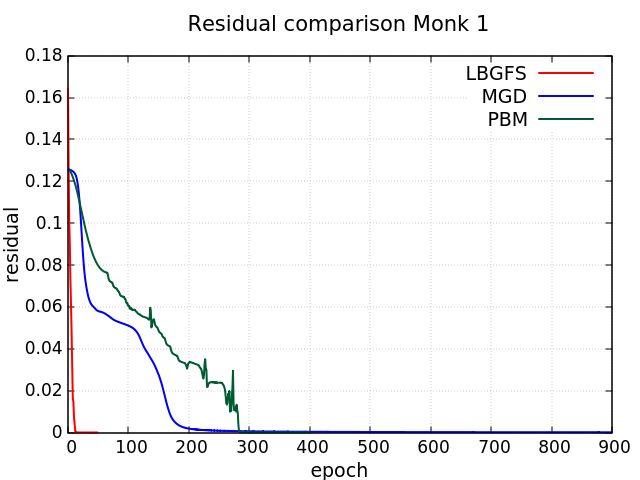
\includegraphics[width=\linewidth]{data/Comparison/Monk1/Monk1_R_Comparison_standard.png}
		%\subcaption{MSE}
	\end{minipage}%
	\begin{minipage}[t]{0.5\linewidth}
		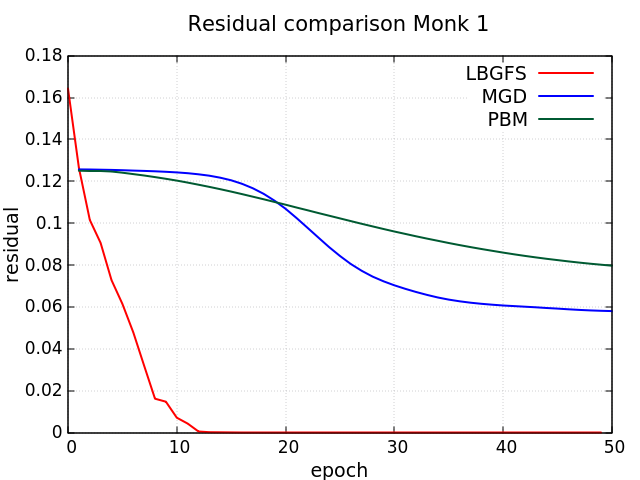
\includegraphics[width=\linewidth]{data/Comparison/Monk1/Monk1_R_Comparison_zoom.png}
		%\subcaption{Accuracy}
	\end{minipage}
	\caption{Residual comparison Monk 1}
	\label{R-Monk1}
\end{figure}
\begin{figure}[H]
	\centering
	\begin{minipage}[t]{0.5\linewidth}
		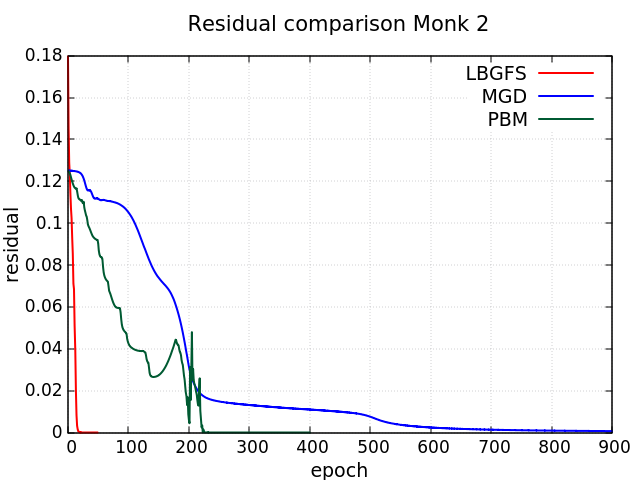
\includegraphics[width=\linewidth]{data/Comparison/Monk2/Monk2_R_Comparison_standard.png}
		%\subcaption{MSE}
	\end{minipage}%
	\begin{minipage}[t]{0.5\linewidth}
		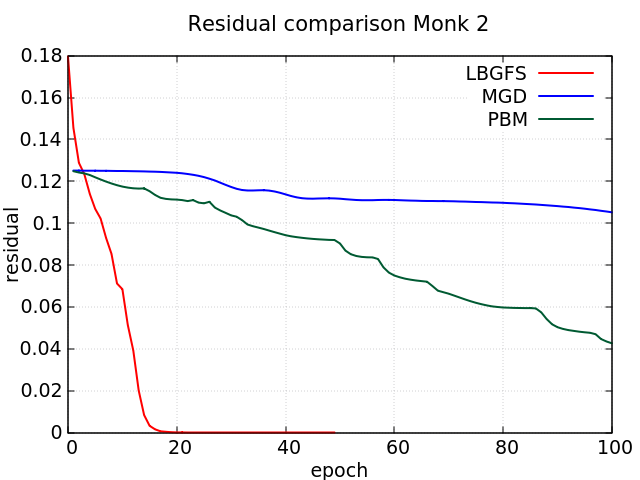
\includegraphics[width=\linewidth]{data/Comparison/Monk2/Monk2_R_Comparison_zoom.png}
		%\subcaption{Accuracy}
	\end{minipage}
	\caption{Residual comparison Monk 2}
	\label{R-Monk2}
\end{figure}
\begin{figure}[H]
	\centering
	\begin{minipage}[t]{0.5\linewidth}
		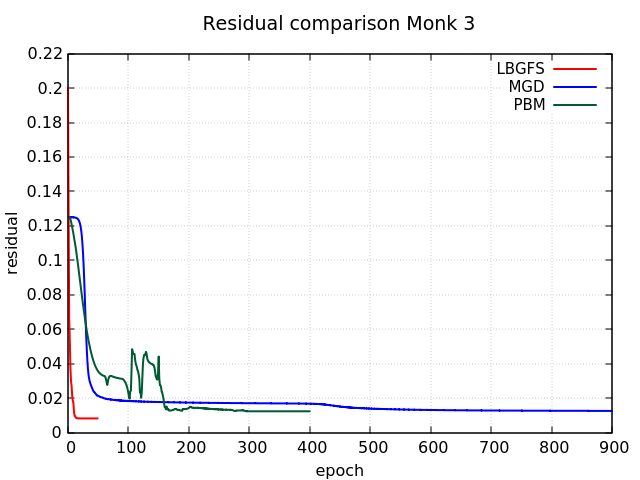
\includegraphics[width=\linewidth]{data/Comparison/Monk3/Monk3_R_Comparison_standard.png}
		%\subcaption{MSE}
	\end{minipage}%
	\begin{minipage}[t]{0.5\linewidth}
		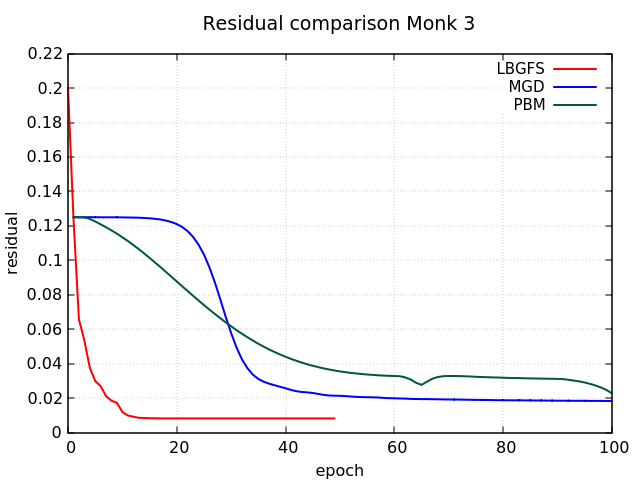
\includegraphics[width=\linewidth]{data/Comparison/Monk3/Monk3_R_Comparison_zoom.png}
		%\subcaption{Accuracy}
	\end{minipage}
	\caption{Residual comparison Monk 3}
	\label{R-Monk3}
\end{figure}
\subsubsection{Computational time}
\begin{figure}[H]
	\centering
	\begin{minipage}[t]{0.5\linewidth}
		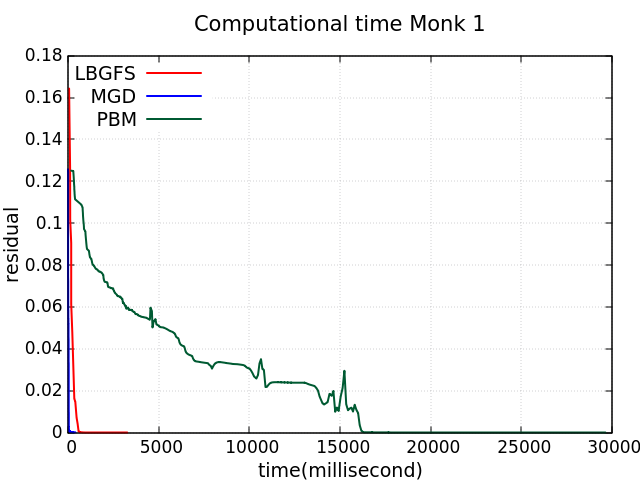
\includegraphics[width=\linewidth]{data/Comparison/Monk1/Monk1_CT_Comparison_standard.png}
		%\subcaption{MSE}
	\end{minipage}%
	\begin{minipage}[t]{0.5\linewidth}
		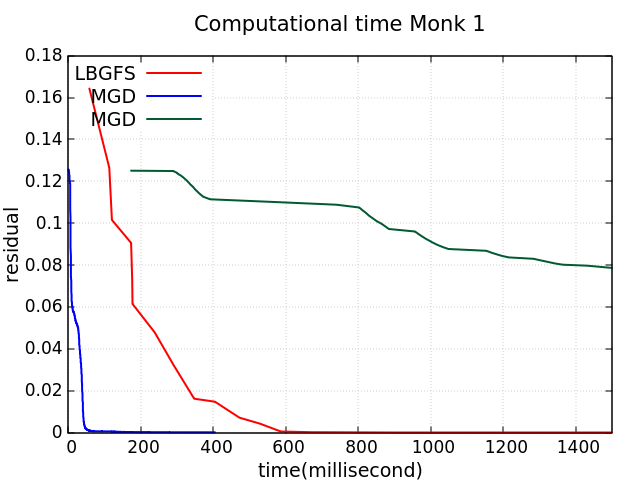
\includegraphics[width=\linewidth]{data/Comparison/Monk1/Monk1_CT_Comparison_zoom.png}
		%\subcaption{Accuracy}
	\end{minipage}
	\caption{Computational time comparison Monk 1}
	\label{CT-Monk1}
\end{figure}
\begin{figure}[H]
	\centering
	\begin{minipage}[t]{0.5\linewidth}
		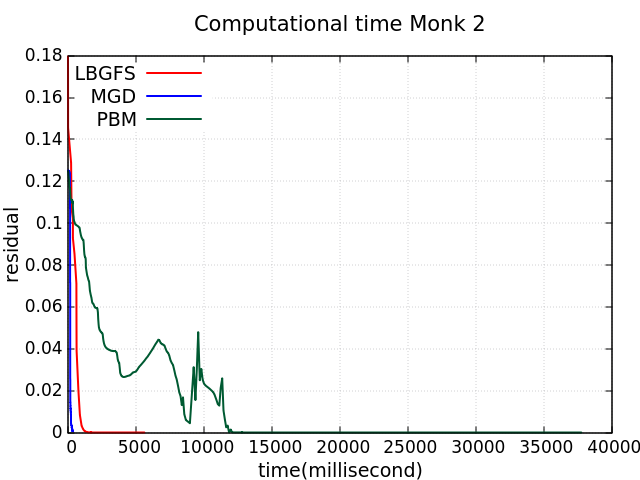
\includegraphics[width=\linewidth]{data/Comparison/Monk2/Monk2_CT_Comparison_standard.png}
		%\subcaption{MSE}
	\end{minipage}%
	\begin{minipage}[t]{0.5\linewidth}
		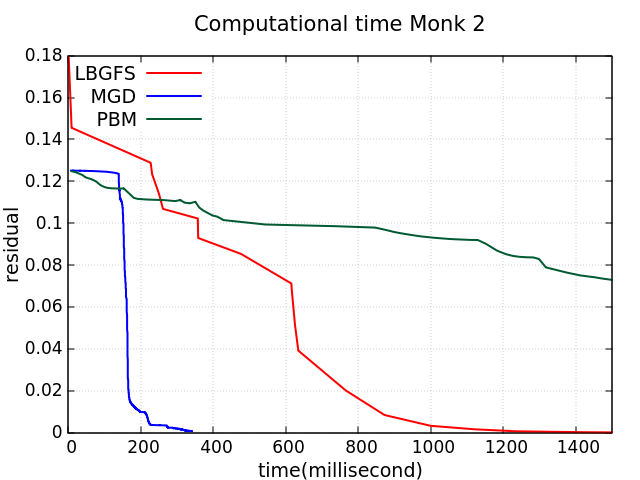
\includegraphics[width=\linewidth]{data/Comparison/Monk2/Monk2_CT_Comparison_zoom.png}
		%\subcaption{Accuracy}
	\end{minipage}
	\caption{Computational time comparison Monk 2}
	\label{CT-Monk2}
\end{figure}
\begin{figure}[H]
	\centering
	\begin{minipage}[t]{0.5\linewidth}
		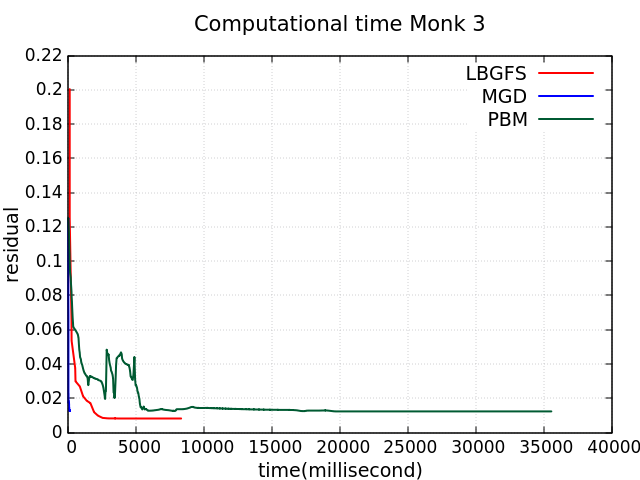
\includegraphics[width=\linewidth]{data/Comparison/Monk3/Monk3_CT_Comparison_standard.png}
		%\subcaption{MSE}
	\end{minipage}%
	\begin{minipage}[t]{0.5\linewidth}
		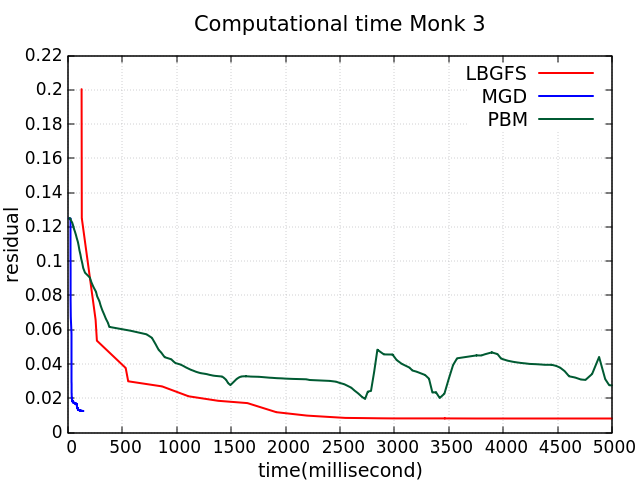
\includegraphics[width=\linewidth]{data/Comparison/Monk3/Monk3_CT_Comparison_zoom.png}
		%\subcaption{Accuracy}
	\end{minipage}
	\caption{Computational time comparison Monk 3}
	\label{CT-Monk3}
\end{figure}



\subsubsection{Convergence Speed}
\begin{figure}[H]
	\centering
	\begin{minipage}[t]{0.5\linewidth}
		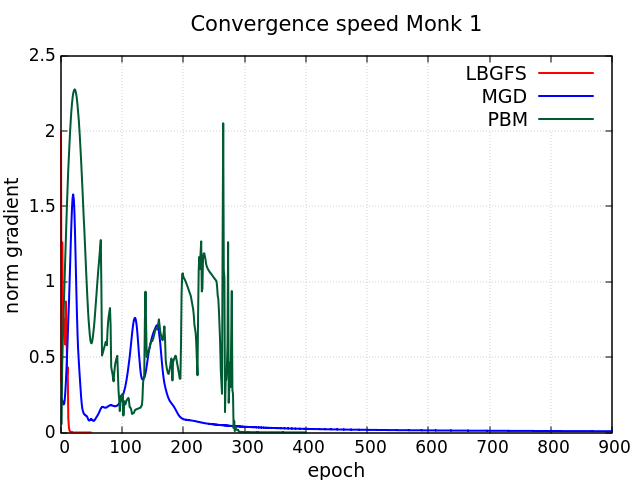
\includegraphics[width=\linewidth]{data/Comparison/Monk1/Monk1_CS_Comparison_standard.png}
		%\subcaption{MSE}
	\end{minipage}%
	\begin{minipage}[t]{0.5\linewidth}
		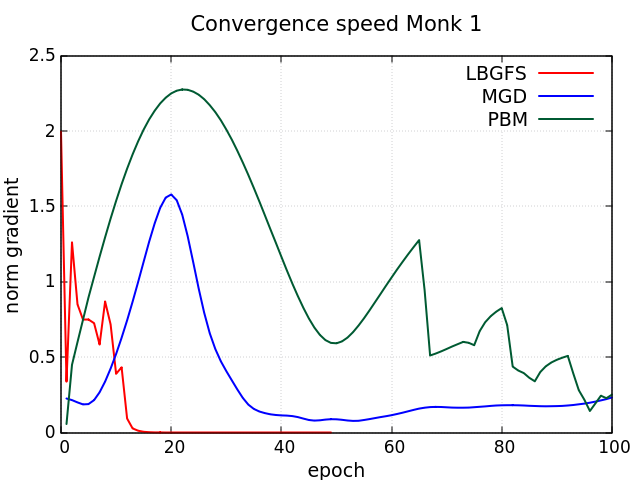
\includegraphics[width=\linewidth]{data/Comparison/Monk1/Monk1_CS_Comparison_zoom.png}
		%\subcaption{Accuracy}
	\end{minipage}
	\caption{Converge speed comparison Monk 1}
	\label{CS-Monk1}
\end{figure}
\begin{figure}[H]
	\centering
	\begin{minipage}[t]{0.5\linewidth}
		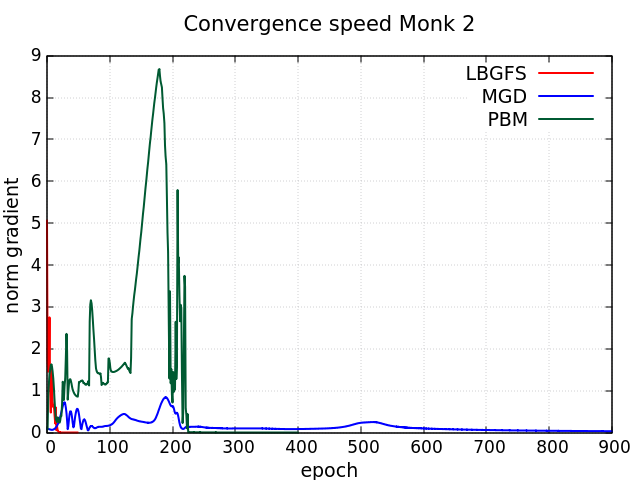
\includegraphics[width=\linewidth]{data/Comparison/Monk2/Monk2_CS_Comparison_standard.png}
		%\subcaption{MSE}
	\end{minipage}%
	\begin{minipage}[t]{0.5\linewidth}
		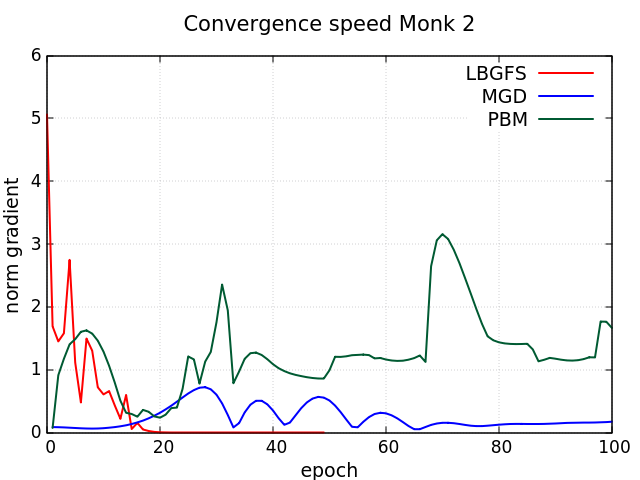
\includegraphics[width=\linewidth]{data/Comparison/Monk2/Monk2_CS_Comparison_zoom.png}
		%\subcaption{Accuracy}
	\end{minipage}
	 \caption{Converge speed comparison Monk 2}
	 \label{CS-Monk2}
\end{figure}
\begin{figure}[H]
	\centering
	\begin{minipage}[t]{0.5\linewidth}
		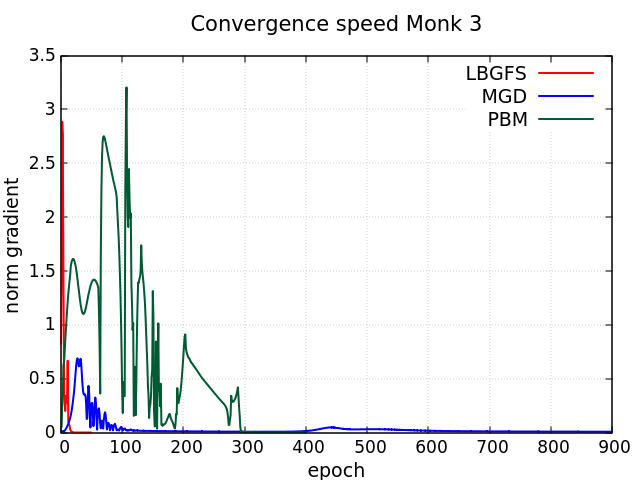
\includegraphics[width=\linewidth]{data/Comparison/Monk3/Monk3_CS_Comparison_standard.png}
		%\subcaption{MSE}
	\end{minipage}%
	\begin{minipage}[t]{0.5\linewidth}
		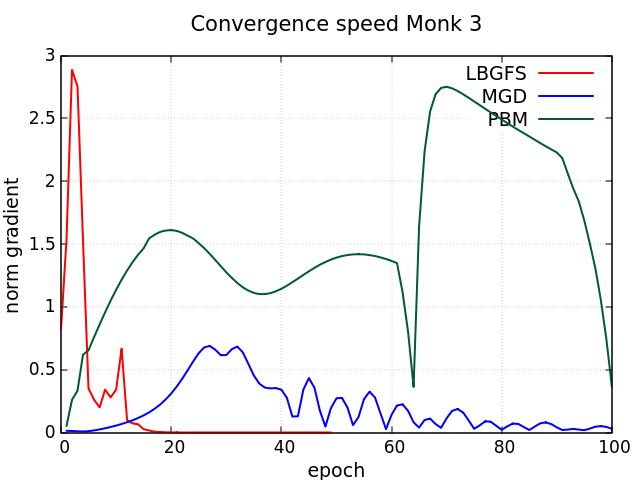
\includegraphics[width=\linewidth]{data/Comparison/Monk3/Monk3_CS_Comparison_zoom.png}
		%\subcaption{Accuracy}
	\end{minipage}
	\caption{Converge speed comparison Monk 3}
	\label{CS-Monk3}
\end{figure}
